\documentclass{standalone}
\usepackage{tikz}
\usetikzlibrary{patterns, positioning}
\usepackage[sfdefault]{ClearSans} %% option 'sfdefault' activates Clear Sans as the default text font
\usepackage[T1]{fontenc}

\begin{document}
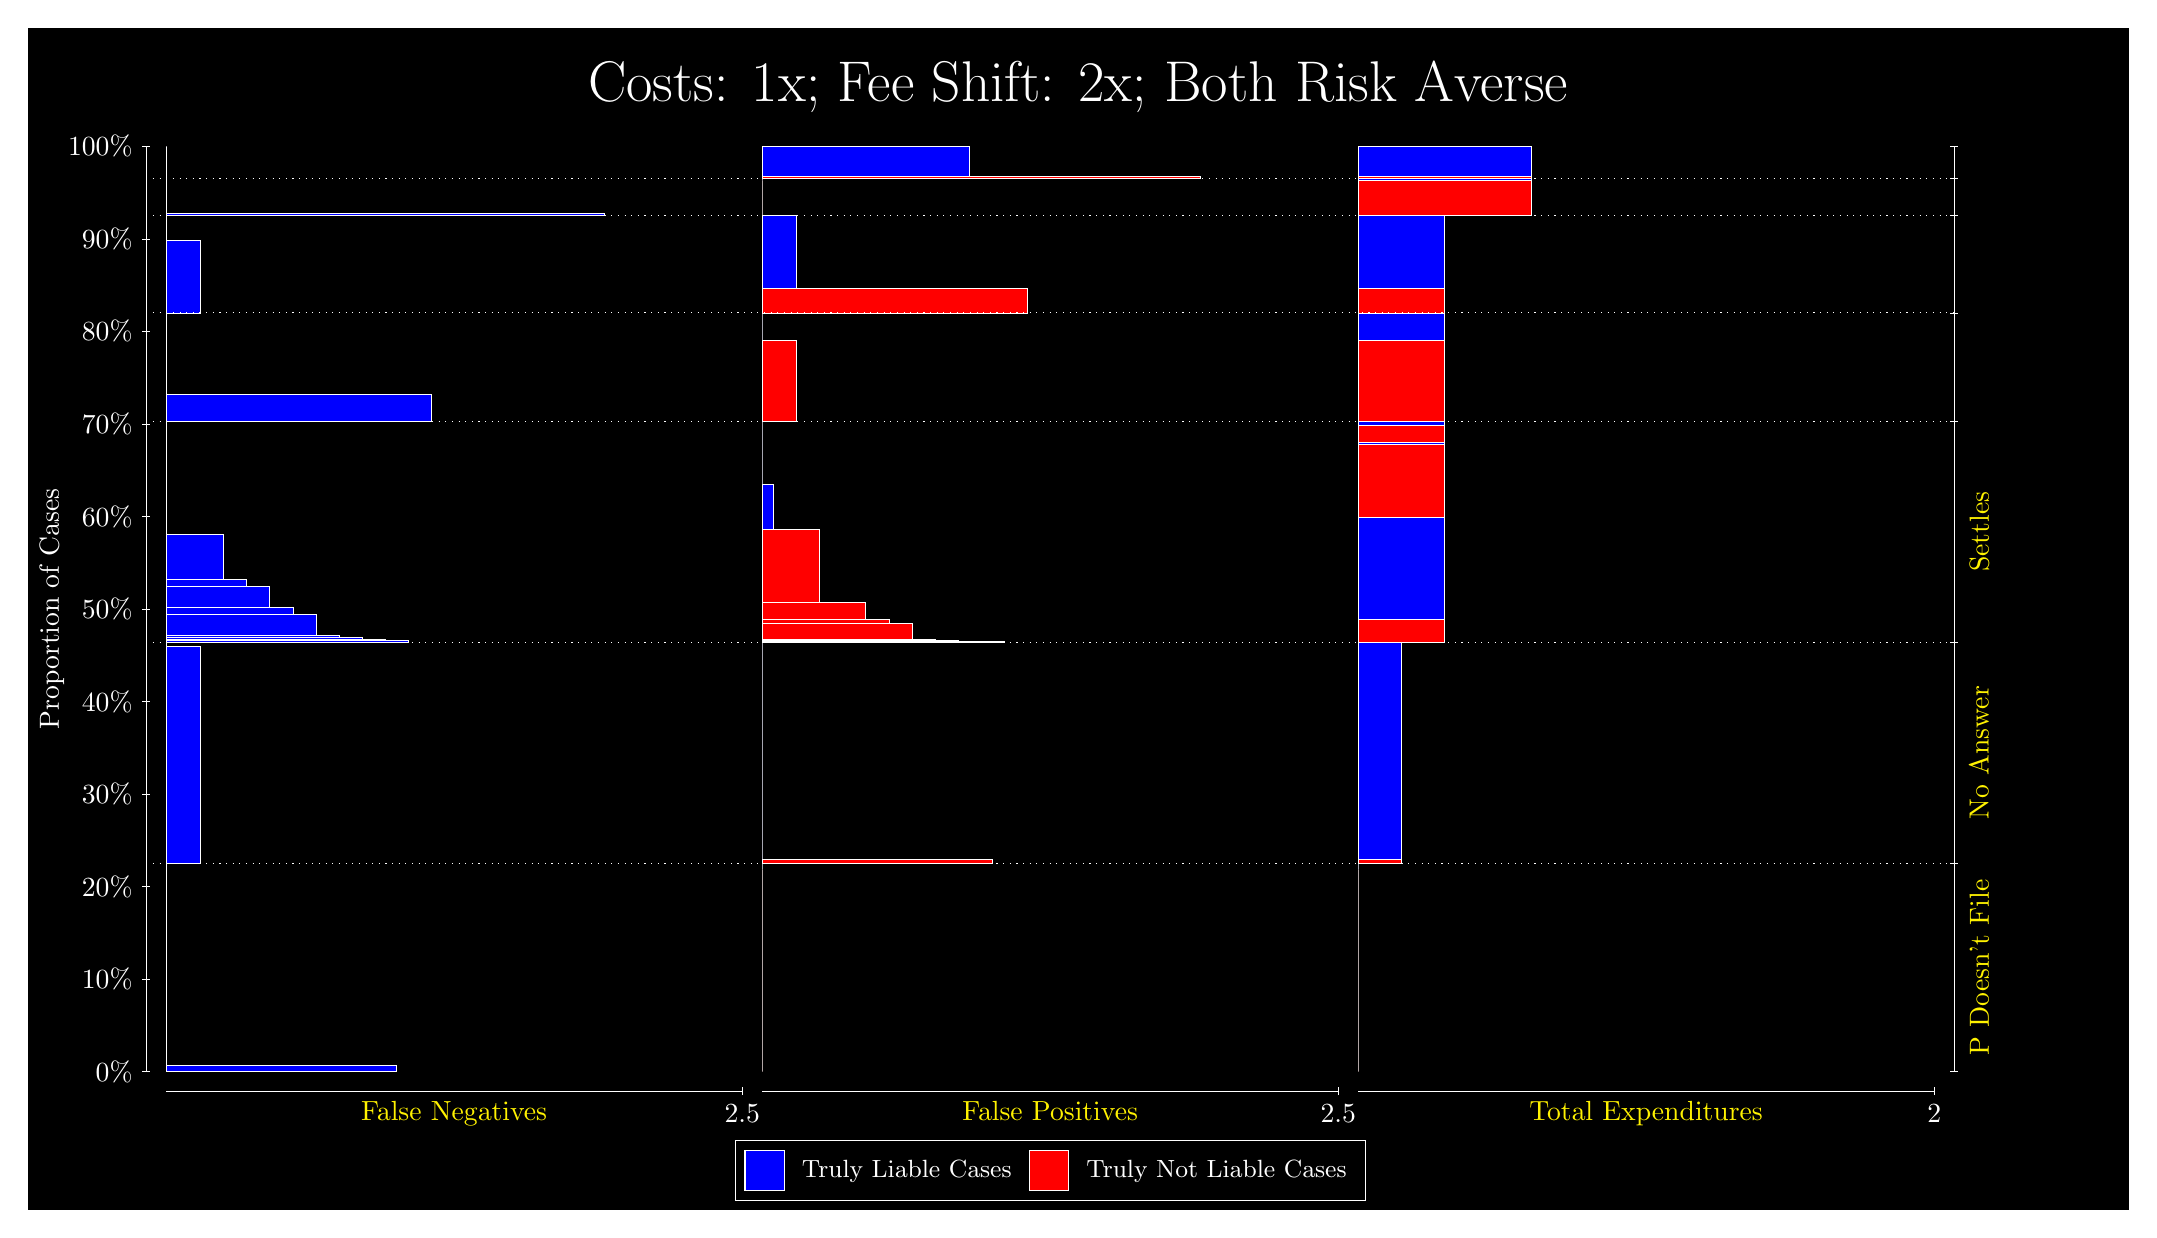
\begin{tikzpicture}
\draw[fill=black] (0,0) rectangle (26.667,15);
\draw[text=white] (0,13.5) rectangle (26.667,15) node[midway] {\huge Costs: 1x; Fee Shift: 2x; Both Risk Averse};
\draw[white, very thin] (1.5,1.75) -- (1.5,13.5);
\node[rotate=90, text=white, anchor=center] at (0.3, 7.625) {Proportion of Cases};
\draw[white, very thin] (1.45,1.75) -- (1.55,1.75);
\node[text=white, anchor=east] at (1.45, 1.75) {0\%};
\draw[white, very thin] (1.45,2.925) -- (1.55,2.925);
\node[text=white, anchor=east] at (1.45, 2.925) {10\%};
\draw[white, very thin] (1.45,4.1) -- (1.55,4.1);
\node[text=white, anchor=east] at (1.45, 4.1) {20\%};
\draw[white, very thin] (1.45,5.275) -- (1.55,5.275);
\node[text=white, anchor=east] at (1.45, 5.275) {30\%};
\draw[white, very thin] (1.45,6.45) -- (1.55,6.45);
\node[text=white, anchor=east] at (1.45, 6.45) {40\%};
\draw[white, very thin] (1.45,7.625) -- (1.55,7.625);
\node[text=white, anchor=east] at (1.45, 7.625) {50\%};
\draw[white, very thin] (1.45,8.8) -- (1.55,8.8);
\node[text=white, anchor=east] at (1.45, 8.8) {60\%};
\draw[white, very thin] (1.45,9.975) -- (1.55,9.975);
\node[text=white, anchor=east] at (1.45, 9.975) {70\%};
\draw[white, very thin] (1.45,11.15) -- (1.55,11.15);
\node[text=white, anchor=east] at (1.45, 11.15) {80\%};
\draw[white, very thin] (1.45,12.325) -- (1.55,12.325);
\node[text=white, anchor=east] at (1.45, 12.325) {90\%};
\draw[white, very thin] (1.45,13.5) -- (1.55,13.5);
\node[text=white, anchor=east] at (1.45, 13.5) {100\%};

\draw[white, very thin] (24.457,1.75) -- (24.457,13.5);
\draw[white, very thin] (24.407,1.75) -- (24.507,1.75);
\node[anchor=west] at (24.407, 1.75) {};
\draw[white, very thin] (24.407,4.3924) -- (24.507,4.3924);
\node[anchor=west] at (24.407, 4.3924) {};
\draw[white, very thin] (24.407,7.2039) -- (24.507,7.2039);
\node[anchor=west] at (24.407, 7.2039) {};
\draw[white, very thin] (24.407,10.008) -- (24.507,10.008);
\node[anchor=west] at (24.407, 10.008) {};
\draw[white, very thin] (24.407,11.386) -- (24.507,11.386);
\node[anchor=west] at (24.407, 11.386) {};
\draw[white, very thin] (24.407,12.627) -- (24.507,12.627);
\node[anchor=west] at (24.407, 12.627) {};
\draw[white, very thin] (24.407,13.094) -- (24.507,13.094);
\node[anchor=west] at (24.407, 13.094) {};
\draw[white, very thin] (24.407,13.5) -- (24.507,13.5);
\node[anchor=west] at (24.407, 13.5) {};

\draw[white, very thin, fill=blue] (1.75,1.75) rectangle (4.6775,1.8255);
\draw[white, very thin, fill=red] (1.75,1.8255) rectangle (1.75,4.3924);
\draw[white, very thin, fill=blue] (1.75,4.3924) rectangle (2.1891,7.1502);
\draw[white, very thin, fill=red] (1.75,7.1502) rectangle (1.75,7.2039);
\draw[white, very thin, fill=blue] (1.75,7.2039) rectangle (4.8239,7.2304);
\draw[white, very thin, fill=blue] (1.75,7.2304) rectangle (4.5312,7.2368);
\draw[white, very thin, fill=blue] (1.75,7.2368) rectangle (4.2384,7.2697);
\draw[white, very thin, fill=blue] (1.75,7.2697) rectangle (3.9457,7.2885);
\draw[white, very thin, fill=blue] (1.75,7.2885) rectangle (3.6529,7.562);
\draw[white, very thin, fill=blue] (1.75,7.562) rectangle (3.3602,7.6398);
\draw[white, very thin, fill=blue] (1.75,7.6398) rectangle (3.0674,7.9073);
\draw[white, very thin, fill=blue] (1.75,7.9073) rectangle (2.7746,8.0062);
\draw[white, very thin, fill=blue] (1.75,8.0062) rectangle (2.4819,8.5701);
\draw[white, very thin, fill=red] (1.75,8.5701) rectangle (1.75,10.008);
\draw[white, very thin, fill=blue] (1.75,10.008) rectangle (5.1167,10.355);
\draw[white, very thin, fill=red] (1.75,10.355) rectangle (1.75,11.386);
\draw[white, very thin, fill=blue] (1.75,11.386) rectangle (2.1891,12.313);
\draw[white, very thin, fill=red] (1.75,12.313) rectangle (1.75,12.627);
\draw[white, very thin, fill=blue] (1.75,12.627) rectangle (7.3123,12.652);
\draw[white, very thin, fill=red] (1.75,12.652) rectangle (1.75,13.094);
\draw[white, very thin, fill=red] (1.75,13.094) rectangle (1.75,13.123);
\draw[white, very thin, fill=blue] (1.75,13.123) rectangle (1.75,13.5);
\draw[white, very thin, fill=red] (9.3189,1.75) rectangle (9.3189,4.317);
\draw[white, very thin, fill=blue] (9.3189,4.317) rectangle (9.3189,4.3924);
\draw[white, very thin, fill=red] (9.3189,4.3924) rectangle (12.246,4.4461);
\draw[white, very thin, fill=blue] (9.3189,4.4461) rectangle (9.3189,7.2039);
\draw[white, very thin, fill=red] (9.3189,7.2039) rectangle (12.393,7.2084);
\draw[white, very thin, fill=red] (9.3189,7.2084) rectangle (12.1,7.2149);
\draw[white, very thin, fill=red] (9.3189,7.2149) rectangle (11.807,7.229);
\draw[white, very thin, fill=red] (9.3189,7.229) rectangle (11.515,7.2337);
\draw[white, very thin, fill=red] (9.3189,7.2337) rectangle (11.222,7.4403);
\draw[white, very thin, fill=red] (9.3189,7.4403) rectangle (10.929,7.4927);
\draw[white, very thin, fill=red] (9.3189,7.4927) rectangle (10.929,7.4945);
\draw[white, very thin, fill=red] (9.3189,7.4945) rectangle (10.636,7.7106);
\draw[white, very thin, fill=red] (9.3189,7.7106) rectangle (10.344,7.7123);
\draw[white, very thin, fill=red] (9.3189,7.7123) rectangle (10.051,8.6419);
\draw[white, very thin, fill=blue] (9.3189,8.6419) rectangle (9.4652,9.2058);
\draw[white, very thin, fill=blue] (9.3189,9.2058) rectangle (9.3189,10.008);
\draw[white, very thin, fill=red] (9.3189,10.008) rectangle (9.758,11.04);
\draw[white, very thin, fill=blue] (9.3189,11.04) rectangle (9.3189,11.386);
\draw[white, very thin, fill=red] (9.3189,11.386) rectangle (12.686,11.7);
\draw[white, very thin, fill=blue] (9.3189,11.7) rectangle (9.758,12.627);
\draw[white, very thin, fill=red] (9.3189,12.627) rectangle (9.3189,13.069);
\draw[white, very thin, fill=blue] (9.3189,13.069) rectangle (9.3189,13.094);
\draw[white, very thin, fill=red] (9.3189,13.094) rectangle (14.881,13.123);
\draw[white, very thin, fill=blue] (9.3189,13.123) rectangle (11.954,13.5);
\draw[white, very thin, fill=red] (16.888,1.75) rectangle (16.888,4.317);
\draw[white, very thin, fill=blue] (16.888,4.317) rectangle (16.888,4.3924);
\draw[white, very thin, fill=red] (16.888,4.3924) rectangle (17.437,4.4461);
\draw[white, very thin, fill=blue] (16.888,4.4461) rectangle (17.437,7.2039);
\draw[white, very thin, fill=red] (16.888,7.2039) rectangle (17.986,7.4927);
\draw[white, very thin, fill=blue] (16.888,7.4927) rectangle (17.986,8.7866);
\draw[white, very thin, fill=red] (16.888,8.7866) rectangle (17.986,9.7162);
\draw[white, very thin, fill=blue] (16.888,9.7162) rectangle (17.986,9.7426);
\draw[white, very thin, fill=red] (16.888,9.7426) rectangle (17.986,9.9623);
\draw[white, very thin, fill=blue] (16.888,9.9623) rectangle (17.986,10.008);
\draw[white, very thin, fill=red] (16.888,10.008) rectangle (17.986,11.04);
\draw[white, very thin, fill=blue] (16.888,11.04) rectangle (17.986,11.386);
\draw[white, very thin, fill=red] (16.888,11.386) rectangle (17.986,11.7);
\draw[white, very thin, fill=blue] (16.888,11.7) rectangle (17.986,12.627);
\draw[white, very thin, fill=red] (16.888,12.627) rectangle (19.083,13.069);
\draw[white, very thin, fill=blue] (16.888,13.069) rectangle (19.083,13.094);
\draw[white, very thin, fill=red] (16.888,13.094) rectangle (19.083,13.123);
\draw[white, very thin, fill=blue] (16.888,13.123) rectangle (19.083,13.5);
\draw[white, dotted] (1.5,4.3924) -- (24.457,4.3924);
\draw[white, dotted] (1.5,7.2039) -- (24.457,7.2039);
\draw[white, dotted] (1.5,10.008) -- (24.457,10.008);
\draw[white, dotted] (1.5,11.386) -- (24.457,11.386);
\draw[white, dotted] (1.5,12.627) -- (24.457,12.627);
\draw[white, dotted] (1.5,13.094) -- (24.457,13.094);
\draw[white, very thin] (1.75,1.5) -- (9.0689,1.5);
\node[text=yellow, anchor=north] at (5.4094, 1.5) {False Negatives};
\draw[white, very thin] (9.0689,1.45) -- (9.0689,1.55);
\node[text=white, anchor=north] at (9.0689, 1.45) {2.5};

\draw[white, very thin] (9.3189,1.5) -- (16.638,1.5);
\node[text=yellow, anchor=north] at (12.978, 1.5) {False Positives};
\draw[white, very thin] (16.638,1.45) -- (16.638,1.55);
\node[text=white, anchor=north] at (16.638, 1.45) {2.5};

\draw[white, very thin] (16.888,1.5) -- (24.207,1.5);
\node[text=yellow, anchor=north] at (20.547, 1.5) {Total Expenditures};
\draw[white, very thin] (24.207,1.45) -- (24.207,1.55);
\node[text=white, anchor=north] at (24.207, 1.45) {2};

\node[text=yellow, centered, rotate=90] at (24.777, 3.0712) {P Doesn't File};
\node[text=yellow, centered, rotate=90] at (24.777, 5.7982) {No Answer};
\node[text=yellow, centered, rotate=90] at (24.777, 8.606) {Settles};





\draw (12.978300999999998,1.5) node[draw=none] (baseCoordinate) {};
\begin{scope}[align=center]
        \matrix[scale=0.5, draw=white, below=0.5cm of baseCoordinate, nodes={draw}, column sep=0.1cm]{
            \node[rectangle, draw, minimum width=0.5cm, minimum height=0.5cm, fill=blue] {}; &
            \node[draw=none, font=\small, text=white] (B) {Truly Liable Cases}; &
            \node[rectangle, draw, minimum width=0.5cm, minimum height=0.5cm, fill=red] {}; &
            \node[draw=none, font=\small, text=white] (B) {Truly Not Liable Cases}; \\
            };
\end{scope}

\end{tikzpicture}
\end{document}